\chapter{Analysis of Possible Blockchain Technologies for INTERLACE}
\label{ch:dlt}

\vspace{-1cm}
\begin{center}
Paolo Dini and Giuseppe Littera
\end{center}

\section{Introduction}
As stated in the INTERLACE proposal, we are not interested in relying on Bitcoin, due its very low performance efficiency ($< 10$ transactions per second, or $[Tx/s]$) and the wastefully high energy requirements of the Proof of Work (PoW) consensus protocol. Bitcoin, however, remains a useful reference point for many blockchain properties and parameters. It is therefore assumed that the reader is already familiar with the basic concepts of the Bitcoin blockchain, which are explained very well in \cite{Antonopoulos2015}.

In the next section we present a few important concepts around which design trade-offs, and in our case selection trade-offs, have been made to arrive at the architecture that we feel is most suitable for INTERLACE and for the Sardex circuit, Hyperledger Fabric. A few more specific details are then presented that concern a small subset of possible Distributed Ledger Technologies (DLTs) in common use, which are summarised at the end of the chapter in a summary table. Thus, the analysis in this chapter forms the basis for the architectural design decisions described in deliverable D2.3 \cite{INTERLACE_D23}.

\section{Basic Concepts}
\subsection{The Blockchain as a Distributed Applications Platform}
The most important innovation implicit in the Bitcoin blockchain is not the creation ``out of thin air'' of a new currency, or the substitution of a central authority for validating a ledger of transactions in this new independent currency with a distributed architecture based on a consensus protocol. These two innovations were the main motivation for creating Bitcoin, but as has been noted by many the potentially more impactful innovation is the blockchain itself. Figure \ref{fig:dapps} proposes a reason why by highlighting the role of the second-generation blockchains such as Ethereum as a distributed, permanent, and immutable memory in enabling a new type of distributed application. The fact that this memory substrate is shared among completely unrelated applications and user groups is interesting from the point of view of the sharing economy, which could be regarded as a third innovation, but the (fourth) innovation that opens up a new space for computer science and software engineering is the fact that the memory is \emph{distributed}, \emph{permanent}, and \emph{immutable}.

As shown in Figure \ref{fig:dapps}, whereas Bitcoin allows only for the simplest kinds of interactions between users and the permanent, distributed, and immutable memory, second-generation blockchains have introduced what looks like a familiar stack: user interface, code, persistence layer. However, the persistence layer is writable only once. A permanent and immutable \emph{shared} history will remain ``on the \emph{shared} record'' forever -- or at least as long as there will be at least one running server hosting the blockchain. Clearly, this is a very special type of application that has never been possible before. If, as Edward De Bono said long ago, memory is the basic mechanism of intelligence \cite{DeBono1969}, this kind of persistence layer could be the start of a collective intelligence with properties and capabilities that are impossible to predict today. For the moment, therefore, we focus on the most obvious use case, a financial information system -- i.e., in the INTERLACE case, the blockchain as the ``mind'' of the real economy. In particular, we wish to define the most appropriate properties of the financial information system and transaction engine for the Sardex circuit.

\begin{figure}[h]
\centering
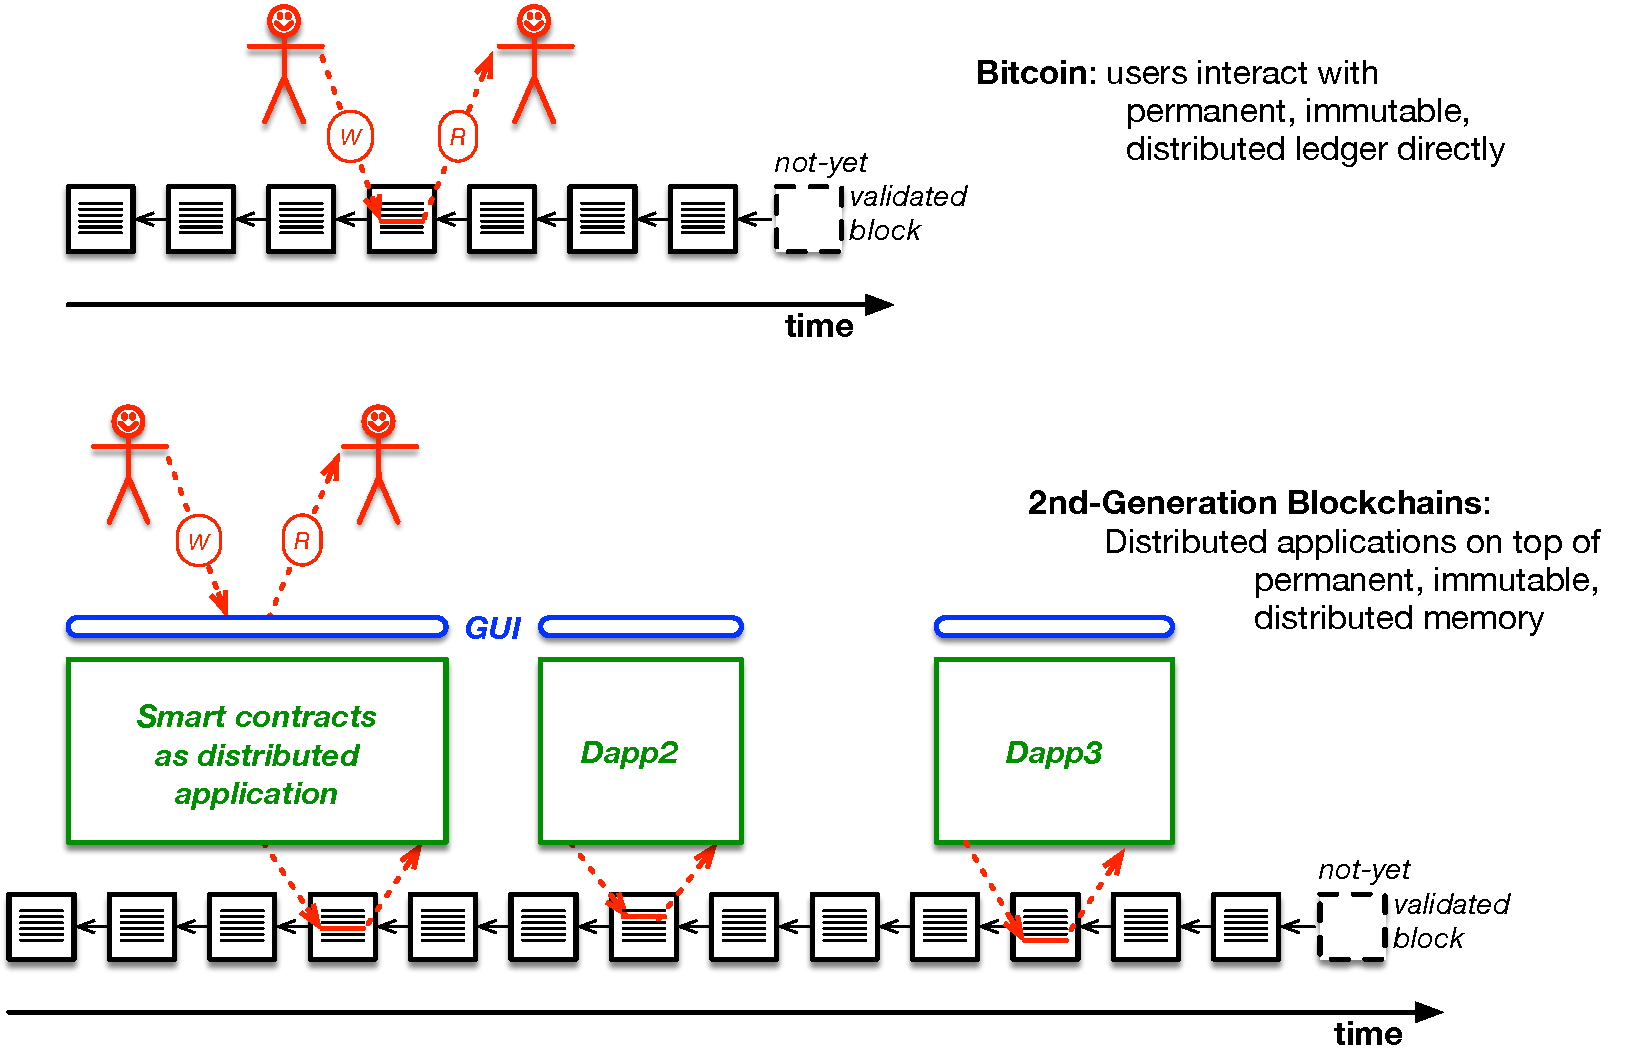
\includegraphics[width=17 cm]{Figures/dapps}
\caption{\bf \small Second-generation blockchains enable a peculiar type of distributed application}
\label{fig:dapps}
\end{figure}

As explained in the Corda technical white paper (\cite{Hearn2016}: 30), the need for organising the transactions into blocks is a consequence of the fact that the rate at which transactions are performed is greater than the rate at which they can be validated by all the peers of a large distributed system with network latencies. The block structure permits the validation of a set of transactions at a time. Since Corda is a permissioned distributed database, it does not need to achieve global consensus and therefore does not need to employ blocks.

\subsection{Deterministic Execution}
As discussed in the Hyperledger technical white paper \cite{AndroulakiEtAl2018}, distributed systems have relied on the state machine replication (SMR) paradigm \cite{Schneider1990} for a few decades. The SMR approach is motivated by the need for redundancy in the provision of services to a given client as a strategy to offset possible faults. Each service request from a client is executed in an identical, deterministic, and asynchronous way by a set of servers, which means that the same operations are executed in the same order by each server, even though not necessarily at the same time. By definition, the correct response is whatever the majority of the servers calculates. Therefore, SMR is resistant also to Byzantine faults, which are malicious and not merely technical. More precisely, an SMR system is $t$-resistant as long as no more than $t$ servers are affected by faults (Byzantine or otherwise) for a total set comprising $2t + 1$ servers. Most blockchains have taken SMR as a starting point, where the set of operations in this case is one block of transactions. In particular, most global consensus algorithms are centred around reaching agreement on the ordering of the transactions in a given block -- hence the name `order-execute' for this type of distributed architecture.

For example, in Bitcoin order-execute involves deterministic sequential execution by each peer, after the first peer has ordered a block, solved the PoW puzzle, and broadcast the block by gossip. The validation of the new block is achieved once every peer has completed and validated the execution. In a public blockchain such as Ethereum a denial-of-service (DoS) attack could be mounted by embedding an infinite loop in the smart contract of one of the transactions. Since it is not possible to determine in general whether or not an algorithm completes (`halting problem'), such a loop could go undetected, leading to a block that cannot be validated and stopping the ability of the blockchain to support future transactions. Ethereum solves this problem by using ``gas'' which, once converted in the cryptocurrency of that blockchain (ether), results in a charge for the execution of transactions.

The low efficiency of sequential execution can be improved upon with parallel execution of unrelated transactions. However, detecting the possible interdependencies is not trivial. Stellar and Holochain seem to have been able to do that.

\subsection{Non-Deterministic Execution}
Non-deterministic execution of smart contracts can lead to forks in the blockchain and is therefore avoided when possible. This can be achieved by means of smart contract languages that are not Turing-complete: they should be expressive enough for the purposes of the blockchain they serve (like Solidity for Ethereum) but not so general as to render complete avoidance of non-determinism impossible. For example, Androulaki et al.\ \cite{AndroulakiEtAl2018} mention a map iterator in Go that is a deterministic operation at the level of the command but hides a non-deterministic implementation in the Go language itself.

\subsection{Confidentiality}
Performing chaincode on all peers may expose details that some peer would rather be kept private. This issue is particularly important in B2B contexts. One possible solution is to replicate the end-state of the calculation (passive replication) rather than the whole calculation (active replication) \cite{AndroulakiEtAl2018}.

\subsection{Native Currency}
The Bitcoin blockchain provides the simplest example of what a native currency is and how it is created. This is done by a miner by writing a transaction to self of (currently) 12.5 BTC at the beginning of the block he/she will then try to validate by finding the nonce that satisfies the puzzle requirement (i.e.\ the hash of the miner's current block with the winning nonce) for the current block. If the miner wins the current PoW puzzle the 12.5 BTC to self will become ``real'' and will be credited to her private key. Many blockchains, like Hyperledger, do not have a native currency. This is what INTERLACE needs because in mutual credit the important concept is not whether or not an \emph{asset} is present but what value someone's credit \emph{balance} has -- a value that can be negative as well as positive.


\subsection{Latency vs.\ Performance in Consensus}
As shown in Figure \ref{fig:consensus_tradeoffs}, the consensus objective can be cast as a trade-off between network latency vs.\ blockchain performance expressed in transactions per second [$Tx/s$] (\cite{vukolic2015}, cited in \cite{AndroulakiEtAl2018}). Stellar here claims the middle ground.


\begin{figure}[h]
\centering
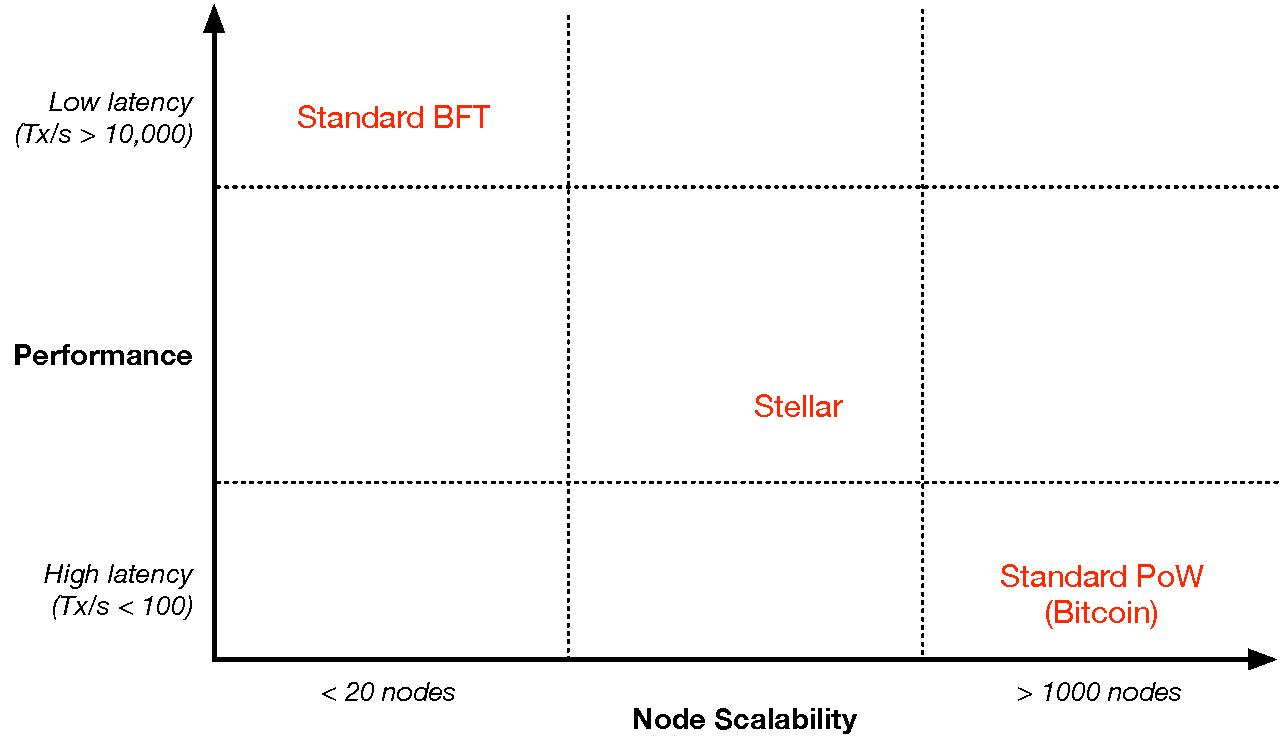
\includegraphics[width=14 cm]{Figures/consensus_tradeoffs}
\caption{\bf \small Network latency-node scalability trade-offs, after \cite{vukolic2015}}
\label{fig:consensus_tradeoffs}
\end{figure}









\section{Brief Summary of Some DLT Technologies}

The INTERLACE team has looked at a number of blockchain technologies, listed here in order of decreasing openness:
\begin{packed_item1}
\item Holochain
\item Ethereum
\item Stellar
\item Quorum (permissioned Ethereum)
\item Hyperledger Fabric
\item Corda
\end{packed_item1}
In this chapter we analyse and discuss them briefly in turn, emphasising the algorithmic, architectural,  mathematical, or financial aspects that are most pertinent to INTERLACE. The frameworks that have made it into this short list are all interesting for one reason or another, and at different points each of them was seriously taken into consideration for adoption. Stellar has an interesting mathematical foundation which is therefore studied and discussed in some detail in the Appendix since mathematical understanding can be transferred to other frameworks. The one that comes closest to the requirements of the Sardex mutual credit system is Hyperledger, as will be shown when discussing the summary table at the end fo the chapter.


\subsection{Holochain}
Holochain is the only DLT we have examined that is agent-centric. This means that it does not attempt to achieve global consistency on the same data on a global ledger, but keeps track of individual peer's data histories.

Holochain is composed of two parts: Holochain proper is the underlying technology -- not a global blockchain but in any case a persistence layer composed of many individual chains \cite{HarrisBrownEtAl2018}, and Holo, the interaction, governance, and financial framework that runs on Holochain.


\subsection{Ethereum}
Asset-centric


\subsection{Stellar}
Stellar is a system for international currency transfer and exchange. Thus, although it has its own native token (Lumens, XLM), this is similar to Ethereum gas in the sense that its main function is to prevent spamming. Thus, the transaction fees to be paid in XLM are very small. The actual assets being exhanged are ``credits'' that correspond to fiat currency that the counterparties wish to trade or exchange. In other words, the units being recorded on the Stellar ledger chain are analogous to the ``statistical Euros'' discussed in  deliverable D3.1 \cite{INTERLACE_D31}.



\subsection{Quorum}
Quorum is a private and permissioned version of Ethereum, optimised for the enterprise.\footnote{\url{https://github.com/jpmorganchase/quorum-docs/blob/master/Quorum_Architecture_20171016.pdf}} \footnote{\url{quorum white paper}}




\subsection{Hyperledger}
The main points of interest of Hyperledger Fabric are \cite{AndroulakiEtAl2018}:


\begin{quote}
\begin{packed_item1}
\item It supports modular consensus protocols, which allows the system to be tailored to particular use cases and trust models.
\item Fabric is the first blockchain system that runs distributed applications written in standard, general-purpose programming languages, without systemic dependency on a native cryptocurrency. This stands in sharp contrast to existing blockchain platforms that require smart contracts to be written in domain-specific languages or rely on a cryptocurrency.
\item Fabric realizes the permissioned model using a portable notion of membership, which may be integrated with industry-standard identity management.
\item Fabric achieves end-to-end throughput of more than 3500 transactions per second in certain popular deployment configurations, with sub-second latency, scaling to well over 100 peers.
\end{packed_item1}
\end{quote}



Hyperledger Indy-Plenum Byzantine Fault Tolerance (PBFT).\footnote{\url{https://github.com/hyperledger/indy-plenum/wiki}} PBFT is based on RBFT: Redundant Byzantine Fault Tolerance
\cite{Aublinetal2013}.



\subsection{Corda}
Corda \cite{Hearn2016} is a permissioned distributed database for banking networks which does not use a blockchain. As explained  in \cite{Hearn2016} (pp 29-30) and mentioned above, the structuring of a blockchain into blocks is a consequence of the difference in time needed to perform a transaction and to reach consensus on that transaction. If in a blockchain like Bitcoin or Ethereum each transaction needed a proof of its validity by global consensus, separately, the number of circulating but not yet proven transactions would be huge and the stable, validated ledger would grow even more slowly. By grouping the transactions into blocks that need to be validated the number of things the network needs to reach consensus on is greatly decreased, and the system reaches some level of efficiency (although much less than VISA -- 7 Tx/s for Bitcoin vs. 57,000 max Tx/s for VISA, for example \cite{Antonopoulos2015}).

Since Corda is permissioned and does not require global consensus, it does not need to group transactions into blocks or to run a consensus protocol. The transactions still need to be verified and validated, which is done by so-called Notaries, after which they are written into the ledger. The ledger is distributed and each node has a copy, but not all nodes see the same information. Visibility of the data is strictly related to whether or not the data is directly related to a particular peer or counterparty in the transaction.

\section{Summary and Comparison Table}
Tables \ref{blockchain_types1} and \ref{blockchain_types2} provide a summary of some of the aspects we have analysed when comparing different blockchain frameworks. The rows are in the same order as the sub-sections of this chapter, from the most open to the most closed frameworks. The order of the topics in each table could perhaps be organised better; they were added on as they were encountered during the literature review. There are two tables only as a question of space, and each table has two sets of rows because the number of properties we examined was too large to fit in a single row. So in fact Tables \ref{blockchain_types1} and \ref{blockchain_types2} should be regarded as a single comparison table. The six frameworks listed represent the best candidates out of the much larger set that was examined.

We ended up choosing Hyperledger, so this table could be used as a way to explain the different trade-offs we encountered in making this choice. For example, as already discussed from the proposal stage of the project, the first choice was to use a private, permissioned platform as the most logical transition from the current centralised relational database to a blockchain for business and trade, where privacy matters.

However, we examined also several public chains because some aspects of the system may benefit from greater transparency. For example, once circuits are established beyond the Euro zone it will become necessary to set up a credit-currency conversion protocol for inter-circuit trades, since each circuit's credit currency will be pegged 1-1 to the local fiat currency of the country where it is located. It may be better to use a public chain for such a currency exchange function, which we envisage as involving a single rate of exchange in both directions and not two separate rates, one for buying and one for selling, as is done normally by the banks and exchange bureaus. In other words, speculation on the currency markets would go against the principles of the circuits, which are built on and in support of the real economy and not the financial economy. Therefore, the greater transparency afforded by a public, permissionless chain would be more appropriate for this function than a private chain.


\begin{table}
\small
\begin{centering}
{\begin{tabular}{| l | c | c | c | c | c | c | c |}
\hline
				& 				& \textbf{Read}			& \textbf{Write}		& \textbf{Data/} 
				& \textbf{Smart}		& \textbf{Smart}			&\textbf{Consensus}\\
\textbf{DLT}		&\textbf{Focus}  	& \textbf{Access} 		& \textbf{Access}	& \textbf{Agent} 
				& \textbf{Contracts} 	& \textbf{Contract}		&\textbf{Model} \\
				& 				& \textbf{} 				& \textbf{} 			& \textbf{} 
				& \textbf{} 			& \textbf{Language(s)}	&\textbf{}  \\
\hline
\hline
\textbf{Holochain}	&General-purpose 			&Public		&Permissionless	&Agent-	&Yes		&Lisp, JS
				&Local 				\\
				&platform 					&DHT		&DHT			&centric	&		&
				& 					\\
\hline
\textbf{Ethereum}	&General-purpose		&Public		&Permissionless	&Data-centric	&Yes		&Solidity	
				&Global, PoS 			 \\
				&platform 				&Chain		&Chain			&			&		&on EVM	
				& 					 \\
\hline
\textbf{Stellar}		&Cross-border 					&Public		&Permissionless	&Data-centric	&Limited	&Limited
				&SCP 				\\
				&exchange 					&			&				&			&		&
				&(FBAS)				\\
\hline

				&Public and  			&			&				&			&		&Solidity
				&Configurable,				\\
\textbf{Quorum} 	&banking  			&Private		&Permissioned		&Data-centric	&Yes		&on EVM
				&voting-based 				\\
			 	&sectors				&			&				&			&		&
				&(PoS, LE, BFT)					\\
\hline
\textbf{Hyperledger}	&Enterprise, B2B		&Private		&Permissioned		&Data-centric	&Yes		&JS, Go
				&Centralised 			\\
 				& \& supply chain		&			&				&			&		&
				& 					\\
\hline
				&Business	 		&			&				&			&		&Bytecode
				&Local state			\\
\textbf{Corda} 		&agrmts between			&Private		&Permissioned		&Data-centric	&Yes		&subset
				&(Notary pools),			\\
		 		&fin. institutions			&			&				&			&		&on JVM
				&pluggable			\\
\hline
\hline
\hline
\hline
				& \textbf{Backup} 		& \textbf{}				&\textbf{Monetary}
				& \textbf{}  			& \textbf{}  			& \textbf{Transaction} 	& \\
\textbf{DLT}		& \textbf{System} 		& \textbf{Interfaces}		&\textbf{Model} 
				& \textbf{Blockchain} 	& \textbf{Immutable} 		& \textbf{Validation} 		& \textbf{Architecture} \\
				& \textbf{} 				& \textbf{}				&\textbf{}
				& \textbf{} 				& \textbf{} 				& \textbf{} 				&\\
\hline
\hline
\textbf{Holochain}	&No			&N/A				&Mutual Credit
				&Individual	&No (link to		&Local to	& \\
				&			&				& 
				&chains 		&repl. code)		&the parties		& \\
\hline
\textbf{Ethereum}	&External		&SQL			&Assets 
				&Yes			&Yes				&Each peer		&Order-Execute \\
				&mirror DB	&				& 
				& 			&				&				& \\
\hline

\textbf{Stellar}		&MySQL,		&Horizon			&Assets
				&Chain of		&Yes				&Global			&Execute-Order-\\
				&PostGres	&				&
				&ledgers		&				&				&Validate\\
\hline
\textbf{Quorum} 	&?			&?				&Assets
				&Yes			&?				&Every node. Data	&Order-Execute\\
			 	&			&				&
				&(Ethereum) 	&				&local to the parties		& \\
\hline
\textbf{Hyperledger}	&Key-value	&SQL			&Adaptable to
				&Yes			&Yes				&Validator				&Execute-Order-\\
 				&store DB		&NoSQL			&Mutual Credit
				&			&				&peers				&Validate \\
\hline
\textbf{Corda} 		&Relational DB	&SQL			&Assets
				&Global ledger	&Yes				&Local to				&Execute-Order-\\
		 		&			&FPML			&
				&locally visible 	&				&the parties			&Validate \\
\hline
\end{tabular}}
\caption{\bf \small Summary table comparing the main properties of different types of blockchain}
\label{blockchain_types1}
\end{centering}
\end{table}

The next property of some interest and relevant is the difference between data-centric and agent-centric blockchains. Holochain is currently the main (and probably only) agent-centric platform. Although its development is not yet completed, it is interesting because it allows the platform to run on each terminal (e.g.\ phone) separately and independently, an architecture which has been dubbed ``fog computing''.\footnote{\url{https://en.wikipedia.org/wiki/Fog_computing}} In Holochain, each agent has its own individual chain. This could be useful for scalability purposes, in the long term, and could also be important as a censorship-resistant alternative to the Bitcoin and Ethereum architectures. In the short term the data-centric approach is sufficient for the objectives of INTERLACE.

Smart contracts are obviously of central importance in a business environment where the business logic needs to be formalised. The consensus model is not as important in a permissioned environment, where the rate of transaction processing and completion takes precedence. Different backup systems and interfaces are available on different chains, but they are not as important discriminating properties.

The most important property after the private/public choice is that the INTERLACE blockchain must support mutual credit. Out of the frameworks we examined, only Holochain and Hyperledger are compatible with mutual credit. Holochain was designed from the ground up as a mutual credit system, whereas Hyperledger can be adapted to become a balance-centric rather than asset-centric chain. In all the others the ``asset'' cannot be a balance that can be either positive or negative: it is assumed to be a positive amount, or a deed, or some quantity of something. Because the Hyperledger assets could be programmed, through smart contracts code, to act as the balance of a mutual credit account, it becomes the obvious choice for INTERLACE.

\begin{table}
\small
\begin{centering}
{\begin{tabular}{| l | c | c | c | c | c | c | c |}
\hline
				& \textbf{Regulatory/} 	& \textbf{Explicit links}	&\textbf{Business}
				& \textbf{Computa-} 		& \textbf{Turing-}		&\textbf{Contract}	& \textbf{Inter-Node}	\\
\textbf{DLT}		& \textbf{Supervisory} 	& \textbf{of SCs to}		&\textbf{flow} 
				& \textbf{tional} 			& \textbf{Complete}		&\textbf{Object}		& \textbf{Comm.} \\
				& \textbf{nodes} 		& \textbf{legal prose}		&\textbf{modelling} 
				& \textbf{Model} 		& \textbf{}				&\textbf{} 			&\\
\hline
\hline
\textbf{Holochain}	&Random				&No			&No 		&?				&?
				&?					&Local \\
				&Peers				&			& 		&				&
				&					& \\
\hline
\textbf{Ethereum}	&No					&No			&No		&Virtual (global)			&No
				&Stateful 				&Global \\
				&					&			&		&Computer		&
				& 					& \\
\hline

\textbf{Stellar}		&No					&No			&No 		&?				&No
				&?					&? \\
\hline
\textbf{Quorum} 	&No					&Yes			&? 		&?				&No
				&?					&Local \\
\hline
\textbf{Hyperledger}	&					&No			&No 		&?				&Yes
				&?					&Global \\
 				&					&			& 		&				&
				&					& \\
\hline
\textbf{Corda} 		&Yes					&Yes			&Yes		&UTXO			&Yes	
				&Stateless			&Local \\
				&					&			&		&				&		
				&					&(Flows) \\
\hline
\hline
\hline
\hline
				& \textbf{Native} 		& \textbf{Transaction}&\textbf{}
				& \textbf{}  			& \textbf{AML}  		& \textbf{} 		& \\
\textbf{DLT}		& \textbf{Token} 		& \textbf{Fees}		&\textbf{Backing} 
				& \textbf{Convertibility}	& \textbf{Compliance} & \textbf{} 		& \textbf{} \\
				& \textbf{} 				& \textbf{}			&\textbf{}
				& \textbf{} 				& \textbf{} 			& \textbf{} 		&\\
\hline
\hline
\textbf{Holochain}	&Yes			&Yes			& Fiat currency,
				&Yes			&			&				& \\
				&(Holo Fuel)	&(Holo Fuel)	&Hosting CPU
				& 			&			&				& \\
\hline
\textbf{Ethereum}	&Yes			&Yes			&No 
				&Yes			&			&				& \\
				&(Ether: ETH)		&(Gas)		& 
				& 			&			&				& \\
\hline

\textbf{Stellar}		&Yes			&Yes, in XLM	&No
				&N/A			&MySQL		&				&\\
				&(Lumens: XLM)&(Very small)	&
				&N/A			&PostGres	&				&\\				
\hline
\textbf{Quorum} 	&No			&Custom-		&N/A
				&Yes			&			&				&\\
			 	&			&izable		&
				& 			&			&				& \\
\hline
\textbf{Hyperledger}	&No			&Custom-		&N/A
				&N/A			&			&				&\\
 				&			&izable		&
				&			&			&				& \\
\hline
\textbf{Corda} 		&No			&Custom-			&N/A
				&N/A			&			&				& \\
		 		&			&izable		&
				& 			&			&				& \\
\hline
\end{tabular}}
\caption{\bf \small Summary table comparing the main properties of different types of blockchain (contd.)}
\label{blockchain_types2}
\end{centering}
\end{table}


Whether or not the technology is a blockchain or a more general DLT was not really an issue. Immutability is important for a public chain but not as much for a private chain since as a matter of course we need to mirror everything onto a relational DB as backup. However, it does imply that private user data cannot be stored on-chain, otherwise we would be violating GDPR requirements (for example, the right to be forgotten). Since Hyperledger is immutable, private data can only be stored in a separate DB, either SQL or key-value. Finally, the execute-order-validate architecture appears to be more suitable for permissioned chains and much faster than most consensus algorithms of the public chains.

The next important feature of interest is Turing-completeness. From a security point of view Turing-completeness is not necessarily a good feature because it implies a larger `attack surface' for malicious hackers. However, it can also imply the use of an established language for the smart contracts. This is the case of Hyperledger, which supports JS, Go, and more recently also Java. In addition, languages that have been developed specifically for smart contracts can have bigger problems. For example, Ethereum's Solidity is not regarded as a properly structured language, and also has security issues of its own.\footnote{See, for example, \url{https://news.ycombinator.com/item?id=14691212}} For these reasons we decided to stick with Hyperledger and the interoperability of well-established languages.

Because Sardex has its own currency, a native token was not important for us. In fact, it would create problems since it would interfere with the financial, economic, and \emph{social} functions of mutual credit \cite{SartoriDini2016}. Anti Money Laundering (AML) and regulatory compliance, on the other hand, are very important for INTERLACE and for Sardex. This was another point in favour of Hyperledger since it exposes a REST interface that can be linked to a regulator's dashboard.



